\documentclass[aspectratio=169]{../latex_main/tntbeamer}  % you can pass all options of the beamer class, e.g., 'handout' or 'aspectratio=43'
\usepackage{dsfont}
\usepackage{bm}
\usepackage[english]{babel}
\usepackage[T1]{fontenc}
%\usepackage[utf8]{inputenc}
\usepackage{graphicx}
\graphicspath{ {./figures/} }
\usepackage{algorithm}
\usepackage[ruled,vlined,algo2e,linesnumbered]{algorithm2e}
\usepackage{hyperref}
\usepackage{booktabs}
\usepackage{mathtools}

\usepackage{amsmath,amssymb}

\DeclareMathOperator*{\argmax}{arg\,max}
\DeclareMathOperator*{\argmin}{arg\,min}

\usepackage{amsbsy}
\newcommand{\vect}[1]{\bm{#1}}
%\newcommand{\vect}[1]{\boldsymbol{#1}}

\usepackage{pgfplots}
\pgfplotsset{compat=1.16}
\usepackage{tikz}
\usetikzlibrary{trees} 
\usetikzlibrary{shapes.geometric}
\usetikzlibrary{positioning,shapes,shadows,arrows,calc,mindmap}
\usetikzlibrary{positioning,fadings,through}
\usetikzlibrary{decorations.pathreplacing}
\usetikzlibrary{intersections}
\pgfdeclarelayer{background}
\pgfdeclarelayer{foreground}
\pgfsetlayers{background,main,foreground}
\tikzstyle{activity}=[rectangle, draw=black, rounded corners, text centered, text width=8em]
\tikzstyle{data}=[rectangle, draw=black, text centered, text width=8em]
\tikzstyle{myarrow}=[->, thick, draw=black]

% Define the layers to draw the diagram
\pgfdeclarelayer{background}
\pgfdeclarelayer{foreground}
\pgfsetlayers{background,main,foreground}

% Requires XeLaTeX or LuaLaTeX
%\usepackage{unicode-math}

\usepackage{fontspec}
%\setsansfont{Arial}
\setsansfont{RotisSansSerifStd}[ 
Path=../latex_main/fonts/,
Extension = .otf,
UprightFont = *-Regular,  % or *-Light
BoldFont = *-ExtraBold,  % or *-Bold
ItalicFont = *-Italic
]
\setmonofont{Cascadia Mono}[
Scale=0.8
]

\renewcommand{\ttdefault}{Cascadia Mono}

% scale factor adapted; mathrm font added (Benjamin Spitschan @TNT, 2021-06-01)
%\setmathfont[Scale=1.05]{Libertinus Math}
%\setmathrm[Scale=1.05]{Libertinus Math}

% other available math fonts are (not exhaustive)
% Latin Modern Math
% XITS Math
% Libertinus Math
% Asana Math
% Fira Math
% TeX Gyre Pagella Math
% TeX Gyre Bonum Math
% TeX Gyre Schola Math
% TeX Gyre Termes Math

% Literature References
\newcommand{\lit}[2]{\href{#2}{\footnotesize\color{black!60}[#1]}}

%%% Beamer Customization
%----------------------------------------------------------------------
% (Don't) Show sections in frame header. Options: 'sections', 'sections light', empty
\setbeamertemplate{headline}{empty}

% Add header logo for normal frames
\setheaderimage{
	% 
\includegraphics[height=\logoheight]{figures/TNT_darkv4.pdf}
	
\includegraphics[height=\logoheight]{../latex_main/figures/Leibniz-AI-Academy_Logo}
	% 
\includegraphics[height=\logoheight]{figures/logo_tntluh.pdf}
}

% Header logo for title page
\settitleheaderimage{
	% 
\includegraphics[height=\logoheight]{figures/TNT_darkv4.pdf}
	
\includegraphics[height=\logoheight]{../latex_main/figures/Leibniz-AI-Academy_Logo}
	% 
\includegraphics[height=\logoheight]{figures/logo_tntluh.pdf}
}

% Title page: tntdefault 
\setbeamertemplate{title page}[tntdefault]  % or luhstyle
% Add optional title image here
%\addtitlepageimagedefault{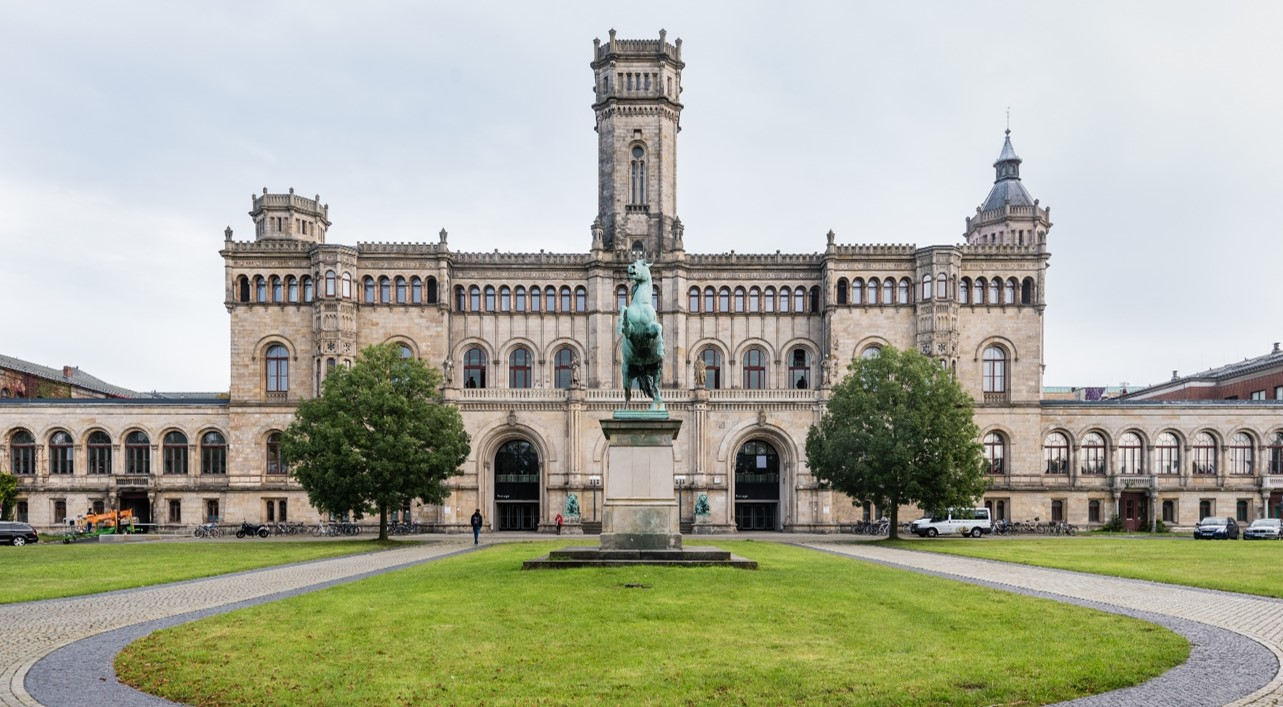
\includegraphics[width=0.65\textwidth]{figures/luh_default_presentation_title_image.jpg}}

% Title page: luhstyle
% \setbeamertemplate{title page}[luhstyle]
% % Add optional title image here
% \addtitlepageimage{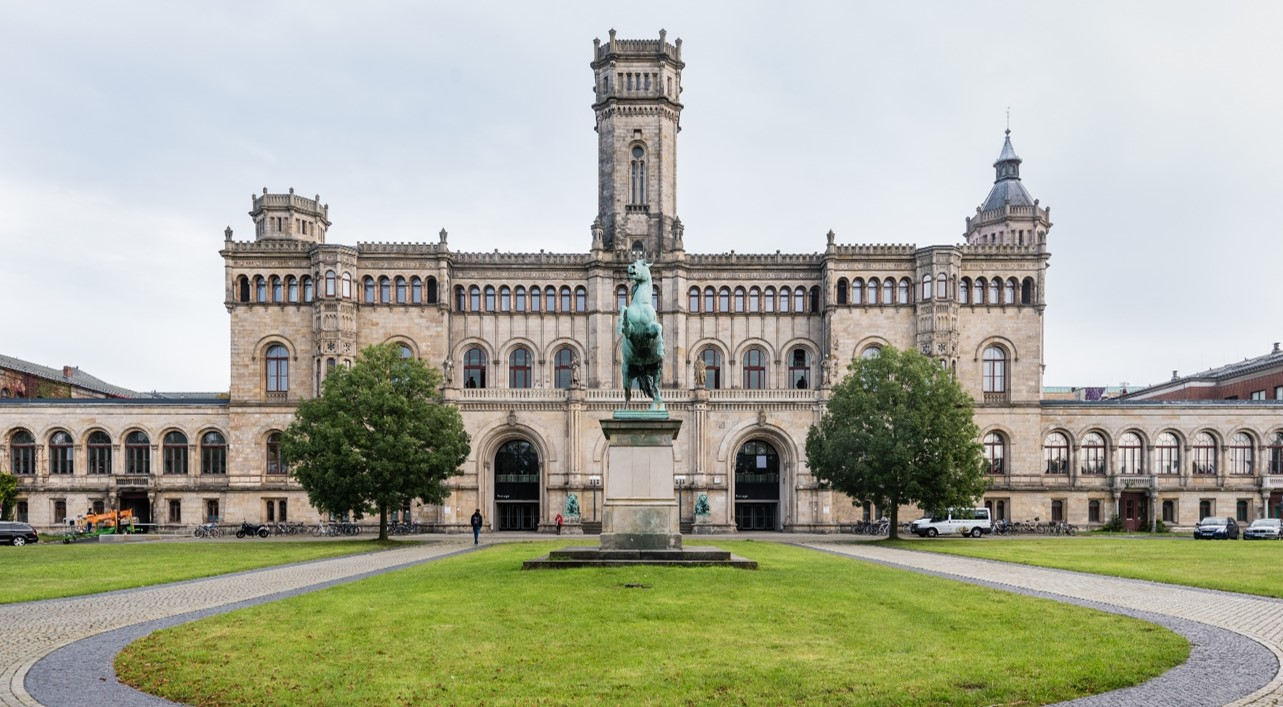
\includegraphics[width=0.75\textwidth]{figures/luh_default_presentation_title_image.jpg}}

\author[Abedjan \& Lindauer]{Ziawasch Abedjan \& \underline{Marius Lindauer}\\[1em]
	%
\includegraphics[height=\logoheight]{../latex_main/figures/luh_logo_rgb_0_80_155.pdf}\qquad
	
\includegraphics[height=\logoheight]{../latex_main/figures/DBIS_Kurzlogo.png}\qquad

\includegraphics[height=\logoheight]{../latex_main/figures/logo_short_highres_black}\qquad

\includegraphics[height=\logoheight]{../latex_main/figures/Leibniz-AI-Academy_Logo}\qquad
%
\includegraphics[height=\logoheight]{../latex_main/figures/L3S.jpg}	
}
\date{\hspace{0.5em} {
\includegraphics[height=1.5em]{../latex_main/figures/Cc-by-nc-sa_icon.svg.png}}; extension of \href{https://ds100.org/fa21/}{[DS100]}
}


%%% Custom Packages
%----------------------------------------------------------------------
% Create dummy content
\usepackage{blindtext}

% Adds a frame with the current page layout. Just call \layout inside of a frame.
\usepackage{layout}


%%% Macros
%\renewcommand{\vec}[1]{\mathbf{#1}}
% \usepackage{bm}
%\let\vecb\bm

\title[Evaluation]{DS: Evaluation}
\subtitle{Validation Metrics for Classification}

\graphicspath{ {./figure/} }
%\institute{}


\begin{document}
	
	\maketitle
	


        \begin{frame}[c]{How to Count for Binary Classification?}
	    \begin{enumerate}
	        \item \alert{Recap}: Choose your validation metric based on your business objective and your data at hand
                \medskip
                \item Let's stay with \alert{binary} classification with possible labels \texttt{positive} and \texttt{negative}
                \item There are four different outcomes if you evaluate a single prediction:
                \begin{description}
                    \item[True Positive~(TP)] The true label was \texttt{positive} and the predicted label was also \texttt{positive}
                    \item[True Negative~(TN)] The true label was \texttt{negative} and the predicted label was also \texttt{negative}
                    \item[False Positive~(FP)] The true label was \texttt{negative} and the predicted label was also \texttt{positive}
                    \item[False Negative~(FN)] The true label was \texttt{positive} and the predicted label was also \texttt{negative}
                \end{description}
	    \end{enumerate}

        These are often represented in a \alert{confusion matrix}:

        \centering
        \begin{tabular}{c|cc}
             & \multicolumn{2}{c}{True labels} \\
             & Positive & Negative \\
             \hline
           Positive & TP & FP \\
           Negative & FN & TN \\
        \end{tabular}

	\end{frame}


        \begin{frame}[c]{Validation Metrics: Accuracy}

        \begin{itemize}
            \item Accuracy is the simplest evaluation metric. It's the proportion of predictions a model got right.
            \item \alert{Pro:} Easy to understand and explain.
            \item \alert{Con:} Doesn't work well with imbalanced classes.
            \item \alert{Application:} Accuracy can be used when the classes are balanced and false positives and false negatives carry the same cost. For instance, an image classification model predicting whether a picture is a cat or a dog can use accuracy as a metric.
        \end{itemize}

        \centering
        \bigskip

        Accuracy = $\frac{{TP + TN}}{{TP + TN + FP + FN}}$

        \medskip
        Balanced Accuracy = $\frac{1}{2} \times \left(\frac{{TP}}{{TP + FN}} + \frac{{TN}}{{TN + FP}}\right)$

	\end{frame}

         \begin{frame}[c]{Validation Metrics: Precision}

        \begin{itemize}
            \item Precision is the proportion of positive predictions that are actually correct.
            \item \alert{Pro:} Useful when the cost of False Positives is high.
            \item \alert{Con:} Doesn't consider False Negatives.
            \item \alert{Application:} Precision is used when the cost of a false positive is high. For example, an email spam filter uses precision because it's more important to ensure that good emails (the "positives") aren't wrongly marked as spam (a false positive). A false positive here means a good email getting into the spam folder which we want to avoid.
        \end{itemize}

        \centering
        \bigskip

        Precision = $\frac{{TP}}{{TP + FP}}$

	\end{frame}

         \begin{frame}[c]{Validation Metrics: Recall}

        \begin{itemize}
            \item Recall is the proportion of actual positives that are correctly classified.
            \item \alert{Pro:} Useful when the cost of False Negatives is high.
            \item \alert{Con:} Doesn't consider False Positives.
            \item \alert{Application:} Recall is used when the cost of a false negative is high. For example, in medical diagnostics, failing to detect a disease when it is present (false negative) can be much more dangerous than diagnosing a healthy patient with the disease (false positive). Therefore, a high recall is desired in such cases.
        \end{itemize}

        \centering
        \bigskip

        Recall = $\frac{{TP}}{{TP + FN}}$

	\end{frame}

         \begin{frame}[c]{Validation Metrics: F1 Score}

        \begin{itemize}
            \item The F1 Score is the harmonic mean of Precision and Recall. It's a balance between Precision and Recall.
            \item \alert{Pro:} Useful when you want to balance Precision and Recall.
            \item \alert{Con:}  Assumes that Precision and Recall are equally important.
            \item \alert{Application:} The F1 Score is used when both false positives and false negatives carry similar cost, and it's important to balance both precision and recall. For example, in information retrieval (like a search engine), it's important both to retrieve as many relevant documents as possible (high recall) and to retrieve as few irrelevant documents as possible (high precision).
        \end{itemize}

        \centering
        \bigskip

        F1 = $2 \times \frac{{Precision \times Recall}}{{Precision + Recall}}$

	\end{frame}

        \begin{frame}[c]{Validation Metrics: F1 Score}

        \vspace{-1em}
        \begin{itemize}
            \item AUC-ROC is the area under the curve when plotting the true positive rate (Recall) against the false positive rate (1-Specificity), for different decision thresholds.
            \item \alert{Pro:}  Useful when you want to evaluate a model's performance across different decision thresholds. Works well with imbalanced classes.
            \item \alert{Con:}  Can be misleading if the classes are highly imbalanced.
            \item \alert{Application:} In credit card fraud detection, the model needs to be sensitive enough to catch as many fraudulent transactions as possible (high recall) while not flagging too many legitimate transactions as fraudulent (high precision). Varying the decision threshold changes the balance between precision and recall, and the AUC-ROC helps find the best balance.
        \end{itemize}

        \centering
        \bigskip

        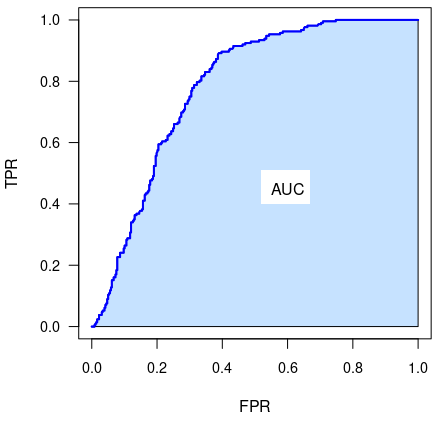
\includegraphics[width=0.18\textwidth]{figure/Basic_AUC_annotated.png}

	\end{frame}
 
 
\end{document}